\chapter{Grafos}
Neste capítulo estão alguns termos e definições relacionadas com teoria de grafos.
\section{Termos e Definições}
\paragraph{Grafo}
Um par ordenado $G = (V,E)$ composto de conjunto de vértices e arestas
\paragraph{Vértice}
Também conhecido como nó. Os elementos principais de um grafo.
\paragraph{Aresta}
Uma linha que conecta dois vértices. Podem ter um peso representando o seu custo.
\paragraph{Adjacente}
Um vértice diz-se adjacente a outro se estiver conectado (incidente) a este por uma aresta.
\paragraph{Grau}
$deg(V)$, $degree(V)$ ou $dG(V)$ é o número de incidências de um vértice, podendo ser um grau pesado (\textit{weighted degree}) se o que for calculado é o peso das arestas.
\paragraph{Grafo orientado}
Um grafo onde todas as arestas são direcionadas de um vértice para o outro.
\paragraph{Grafo não orientado}
Um grafo onde todas as restas são bidirecionais.
\paragraph{Comunidade}
Uma partição do grafo onde os nós estão densamente conectados entre si.
\paragraph{Sub-grafo}
Um sub-grafo é um grafo em que o seu conjunto de vértices e arestas está contido no conjunto de um outro grafo.
\paragraph{$k$-Core}
A $k$-Core de um grafo é um sub-grafo em que todos os vértices tenham um grau de ao menos $k$. Exemplificado da figura~\ref{fig:gekCore}.

\begin{figure}
\centering
\caption{Decomposição k-Core de um grafo, tirada de~\cite{kCoreDis}}
\label{fig:gekCore}
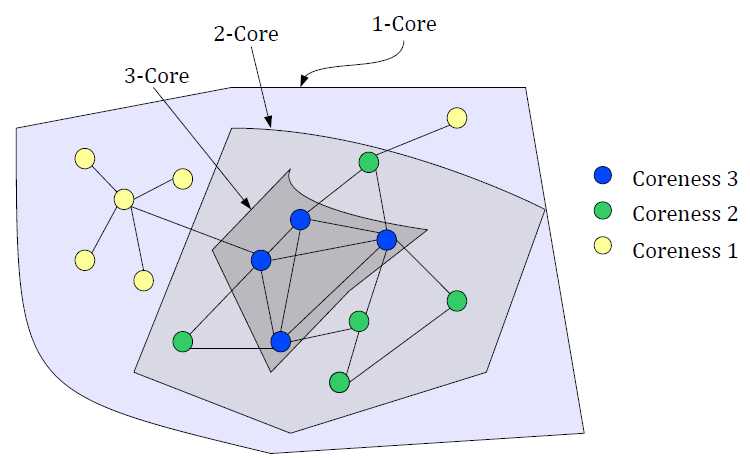
\includegraphics[width=90mm]{kCoreExample}
\end{figure}

\paragraph{Modularidade}
Deteção de uma comunidade de um grafo envolve a partição deste em comunidades de nós densamente conectados. A modularidade mede a densidade das arestas dentro das comunidades em comparação com aquelas entre comunidades e é usada para saber a qualidade da partição de um grafo em comunidades criadas por um algoritmo. 


Modularidade de uma partição para grafos com pesos nas arestas:

\begin{equation}
Q = \frac{1}{2m} \sum_{i,j} [ A_{ij} - \frac{k_i k_j}{2m} ] \delta(c_i ,c_j)
\label{eq:MN}
\end{equation}


\begin{itemize}
	\item $A_{ij}$ é o peso da aresta entre $i$ e $j$.
	\item $k_i = \sum_j A_{ij}$ é a soma do peso de todas as arestas de $i$, com o mesmo significado para $k_j$.
	\item $c_i$ é a comunidade de $i$, com o mesmo significado para $c_j$.
	\item $\delta(c_i,c_j)$ é a igualdade entre $c_i$ e $c_j$ ( os dois vértices serem da mesma comunidade).
	\item $m = \frac{1}{2}\sum_{ij} A_{ij}$ é a soma do peso de todas as arestas %metade porque consideram que 
%o peso das arestas será calculado duas vezes, por cada vértice. Logo é necessário dividir.
\end{itemize}






